\chapter{Rappels sur les nombres}\label{ChNbEntiersDecimaux}

\begin{acquis}
\begin{itemize}
\item lire et écrire des nombres décimaux en chiffres;
\item déterminer le chiffre des dizaines, des unités, des dixièmes, des centièmes… d'un nombre décimal;
\item déterminer le nombre de dizaines, d’unités, de dixièmes, de centièmes… d'un nombre décimal;
\item connaître la définition d'une fraction et le vocabulaire s'y rapportant;
\item savoir passer de l'écriture décimale à une écriture fractionnaire d'une quantité et inversement;
\item placer des nombres décimaux sur une droite graduée et lire les abscisses de nombres décimaux placés sur une droite graduée (sous forme décimale ou fractionnaire);
\item classer des nombres décimaux par ordre croissant et décroissant en utilisant les symboles < ou >;
\item encadrer un nombre décimal à une précision donnée;
\item déterminer l'arrondi d'un nombre décimal à une précision donnée;
\end{itemize}
\end{acquis}

\cours
\section{Le système décimal}

% remarque : pour qu'un mot se retrouve dans le lexique : \MotDefinition{asymptote horizontale}{}
Les règles et conventions qui permettent d'écrire et de lire les nombres forment ce qu'on appelle un \textbf{système de numération}. Nous utilisons le système décimal, de base dix.

\begin{aconnaitre}
Pour écrire les chiffres dans le système décimal, il nous faut dix symboles, appelés des \emph{chiffres}. Ces chiffres sont :
\[ 0\,;\,1\,;\,2\,;\,3\,;\,4\,;\,5\,;\,6\,;\,7\,;\,8\,;\,9  \]
Il arrive parfois qu'on confonde \textbf{\MotDefinition{chiffre}{}} et \textbf{\MotDefinition{nombre}{}}. On peut faire l'analogie avec l'écriture d'une langue en affirmant que les \textbf{\textcolor{H1}{chiffres}} sont des \textbf{\textcolor{H1}{lettres}} et que les \textbf{\textcolor{H1}{nombres}} sont des \textbf{\textcolor{H1}{mots}}. Ainsi, 13 est un nombre qui s'écrit avec les chiffres 1 et 3.
\end{aconnaitre}

%%%%%%%%%%%%%%%%%%%%%%%%%%%%%%%%%%%%%%%%%%%%%%%%%%%%%%%%%%%%%%%%%%%%%%%%%%%
\prof
{Il est très important que les élèves fassent la différence entre chiffre et nombre pour la suite du chapitre. Ils ont sans doute appris autre chose à l'école primaire donc il faut découstruire ce faux-savoir.}
%%%%%%%%%%%%%%%%%%%%%%%%%%%%%%%%%%%%%%%%%%%%%%%%%%%%%%%%%%%%%%%%%%%%%%%%%%%

Un \textbf{\textcolor{C2}{nombre décimal}} est un nombre qui s'écrit en deux parties séparées par une virgule (écriture décimale).

\hspace{2em}\textbullet\hspace{.25em} la partie entière, à gauche de la virgule. Elle correspond au nombre d'unités entières contenues dans le nombre.

\hspace{2em}\textbullet\hspace{.25em} la partie décimale, à droite de la virgule. Elle correspond à une portion d'unité supplémentaire.

De ce fait:

\begin{center}
\textbf{\textcolor{C2}{nombre décimal = partie entière + partie décimale}}
\end{center}

Un nombre entier est caractérisé par le fait qu'il n'a pas de partie décimale (on omet alors la virgule).


\begin{methode*1}[Tableau des nombres]
\begin{exemple*1}

Soit le nombre 34 567,19

\hspace{2em}\textbullet\hspace{.25em} Partie entière: 34 567
 
\hspace{2em}\textbullet\hspace{.25em} Partie décimale: 0,19


\end{exemple*1}

\exercice

Soit le nombre 10,153.

\hspace{2em}\textbullet\hspace{.25em}Partie entière: \dotfill

\hspace{2em}\textbullet\hspace{.25em} Partie décimale:\dotfill

\exercice

Compléter le tableau suivant pour les nombres 10,01 ; 0,037 ; 200 000 042 000.

\vspace{2em}

\begin{ttableau}{\linewidth}{19}
\hline
\multicolumn{3}{|c|}{milliards} & \multicolumn{3}{c|}{millions} & \multicolumn{3}{c|}{mille} & 
\multicolumn{3}{c|}{unités} & 
\multirow{2}{*}{\parbox{\linewidth}{ \vspace{1.5cm} \textcolor{B1}{  \textbf{,} }  }} &  %ADD PARBOX !!
\multirow{2}{*}{\rotatebox{90}{\phantom{dixièmes}}} &
\multirow{2}{*}{\rotatebox{90}{\phantom{centièmes}}} & 
\multirow{2}{*}{\rotatebox{90}{\phantom{millièmes}}} & 
\multirow{2}{*}{\rotatebox{90}{\phantom{dix-millièmes}}} & 
\multirow{2}{*}{\rotatebox{90}{\phantom{cent-millièmes}}} &
\multirow{2}{*}{\rotatebox{90}{\phantom{millionièmes}}} \\ \cline{1-12}
\rotatebox{90}{\phantom {centaines de ...}} & 
\rotatebox{90}{\phantom {dizaines de ...}} & 
\rotatebox{90}{\phantom {unités de ...}} &
\rotatebox{90}{\phantom {centaines de ...}} & 
\rotatebox{90}{\phantom {dizaines de ...}} & 
\rotatebox{90}{\phantom {unités de ...}} &
\rotatebox{90}{\phantom {centaines de ...}} & 
\rotatebox{90}{\phantom {dizaines de ...}} & 
\rotatebox{90}{\phantom {centaines de ...}} &
\rotatebox{90}{\phantom {dizaines de ...}} & 
\rotatebox{90}{\phantom {unités de ...}} & 
 & & & & & &       &   \\ \hline  % ADD EXTRA & ON THIS LINE B4 \\ \hline !!
& & & & & 3 & 0 & 2 & 7 & 4 & 6 & 2 & \textcolor{B1}{\textbf{,}} & 0 & 0 & 0 & 0 & 0 & 0 \\ \hline
& & & & & & & & & & & & \textcolor{B1}{\textbf{,}} & & & & & &\\ \hline
& & & & & & & & & & & & \textcolor{B1}{\textbf{,}} & & & & & &\\ \hline
& & & & & & & & & & & & \textcolor{B1}{\textbf{,}} & & & & & &\\ \hline
\end{ttableau}
\end{methode*1}

\begin{remarque}

\hspace{2em}\textbullet\hspace{.25em} La partie décimale est toujours finie: on peut compter les chiffres après la virgule.

\hspace{2em}\textbullet\hspace{.25em} Lorsque la partie décimale n'est pas finie, on a un nombre infini qui n'est PAS un nombre décimal.

\hspace{2em}\textbullet\hspace{.25em} Lorsque la partie décimale ne comporte que des 0, on les supprime avc la virgule et on parle alors de \textbf{\textcolor{C2}{nombre entier}}.
\end{remarque}
%%%%%%%%%%%%%%%%%%%%%%%%%%%%%%%%%%%%%%%%%%%%%%%%%%%%%%%%%%%%%%%%%%%%%%%%%%%

\section{Nombre en écriture fractionnaire}
Le système décimal peut se représenter ainsi:

\begin{center}
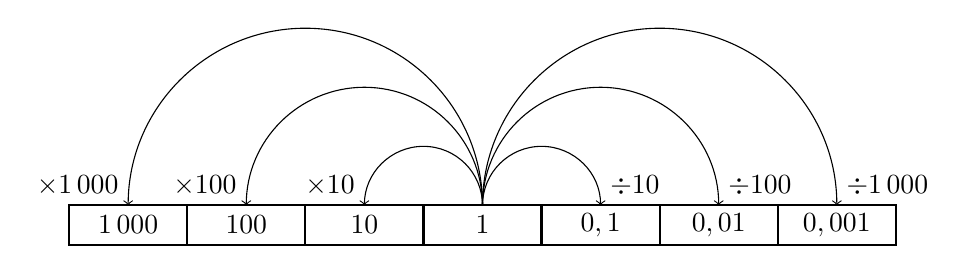
\begin{tikzpicture}[scale=0.5]
\foreach \x in {0,1,...,6} \draw[thick] (-1.5+3*\x,-0.5) rectangle (1.5+3*\x,0.5);
\draw (0,0) node {$1\,000$};
\draw (3,0) node {$100$};
\draw (6,0) node {$10$};
\draw (9,0) node {$1$};
\draw (12,0) node {$0,1$};
\draw (15,0) node {$0,01$};
\draw (18,0) node {$0,001$};
\draw[->] (9,0.5) arc (0:180:4.5) node[above left] {$\times 1\,000$};
\draw[->] (9,0.5) arc (0:180:3) node[above left] {$\times 100$};
\draw[->] (9,0.5) arc (0:180:1.5) node[above left] {$\times 10$};

\draw[->] (9,0.5) arc (180:0:4.5) node[above right] {$\div 1\,000$};
\draw[->] (9,0.5) arc (180:0:3) node[above right] {$\div 100$};
\draw[->] (9,0.5) arc (180:0:1.5) node[above right] {$\div 10$};
\end{tikzpicture}
\end{center}

Dans la partie entière $\left\lbrace
	\begin{matrix}
	\text{Une dizaine c'est l'unité prise 10 fois.}\\
	\text{Une centaine c'est l'unité prise 100 fois.}\\
	\text{Un millier c'est l'unité prise 1 000 fois.}\\
	\end{matrix}
\right.$ 

Dans la partie décimale $\left\lbrace
	\begin{matrix}
	\text{Une dixième c'est l'unité divisée par 10. Cela peut s'écrire} \frac{1}{10}. \\
	\text{Un centième c'est l'unité divisée par 100. Cela peut s'écrire} \frac{1}{100}. \\
	\text{Un millième c'est l'unité divisée par 1 000. Cela peut s'écrire} \frac{1}{1000}.
	\end{matrix}
\right.$

		\subsection{Ecriture fractionnaire d'un nombre}
\begin{aconnaitre}
Le "partage" de l'unité peut s'écrire \textbf{sous forme fractionnaire}.

Ainsi $\frac{1}{5}$ se lit "un cinquième". Cette fraction représente l'unité divisée en 5 parts égales. \\

\begin{center}
\begin{tikzpicture}[scale=0.5]
\fill[white] (0,0) rectangle (5,5);        % Specify colour
\fill[gray!40] (0,0) rectangle (1,5);        % Specify colour
\draw[thick] (0,0) -- (5,0) -- (5,5) -- (0,5) -- cycle;
\foreach \x in {1,2,3,4} \draw[thick] (\x,0) -- (\x,5);

\draw (2.5,0) node[below] {$\dfrac{1}{5}=0,2$};
\end{tikzpicture}
\end{center}

$\frac{1}{5}$ est \textbf{l'écriture fractionnaire} alors que 0,2 est \textbf{l'écriture décimale} \underline{d'une même quantité}.
\end{aconnaitre}

\begin{methode*1}[Comprendre les fractions]
	\begin{exemple*1}
\vspace{0.5cm}	
	
Dans le nombre $\frac{3}{5}$ l'unité est divisée en 5 parts égales et on a pris trois parts: $3\times \frac{1}{5}$.
\begin{center}
\begin{tikzpicture}[scale=0.5]
\fill[white] (0,0) rectangle (5,5);        % Specify colour
\fill[gray!40] (0,0) rectangle (3,5);        % Specify colour
\draw[thick] (0,0) -- (5,0) -- (5,5) -- (0,5) -- cycle;
\foreach \x in {1,2,3,4} \draw[thick] (\x,0) -- (\x,5);

\draw (2.5,0) node[below] {$\dfrac{3}{5}=0,6$};
\end{tikzpicture}
\end{center}

Le nombre du bas, celui qui indique le nombre de parts dans l'unité, s'appelle \textbf{\textcolor{C2}{le dénominateur}}.\\
Le nombre du haut, celui qui indique le nombre de parts, s'appelle \textbf{\textcolor{C2}{le numérateur}}.
\end{exemple*1}

\exercice

Dans chaque cas, donner l'écriture décimale correspondante:

$\frac{1}{100}$=\dotfill \\
$\frac{3}{4}$=\dotfill \\
$\frac{7}{10}$=\dotfill \\
$\frac{12}{25}$=\dotfill \\
$\frac{23}{50}$=\dotfill

\exercice

Dans chaque cas, donner une écriture fractionnaire correspondante:

0,5=\dotfill \\
0,32=\dotfill \\
0,04=\dotfill \\
0,25=\dotfill

\end{methode*1}

\begin{remarque}
Il est important de savoir calculer avec des écritures fractionnaires car certaines quantités ne peuvent pas s'écrire sous forme décimale.\end{remarque}

		\subsection{Partie entière et nombres en écriture fractionnaire}

Parfois, il arrive qu'on "garde" tellement de morceaux d'unité, qu'on arrive à reconstituer une ou plusieurs unités.

\begin{methode*1}[Fraction supérieure à 1]
	\begin{exemple*1}
\vspace{0.5cm}	
	
Prenons la fraction: $\frac{12}{5}$.\\
Cela signifie qu'on a gardé 12 parts égales à $\frac{1}{5}$.\\
Avec 5 parts égales à $\frac{1}{5}$, on peut faire une unité. Donc avec 12 parts de $\frac{1}{5}$, on peut constituer 2 unités et il restera 2 parts de $\frac{1}{5}$ c'est à dire $\frac{2}{5}$.\\
On peut donc dire que $\frac{12}{5}$=2+$\frac{2}{5}$=2,4.

\begin{center}
\begin{tikzpicture}[scale=0.5]
\fill[white] (0,0) rectangle (5,5);        % Specify colour
\fill[gray!40] (0,0) rectangle (5,5);        % Specify colour
\draw[thick] (0,0) -- (5,0) -- (5,5) -- (0,5) -- cycle;
\foreach \x in {1,2,3,4} \draw[thick] (\x,0) -- (\x,5);

\fill[white] (6,0) rectangle (11,5);        % Specify colour
\fill[gray!40] (6,0) rectangle (11,5);        % Specify colour
\draw[thick] (6,0) -- (11,0) -- (11,5) -- (6,5) -- cycle;
\foreach \x in {1,2,3,4} \draw[thick] (6+\x,0) -- (6+\x,5);

\fill[white] (12,0) rectangle (17,5);        % Specify colour
\fill[gray!40] (12,0) rectangle (14,5);        % Specify colour
\draw[thick] (12,0) -- (17,0) -- (17,5) -- (12,5) -- cycle;
\foreach \x in {1,2,3,4} \draw[thick] (12+\x,0) -- (12+\x,5);

\draw (8.5,0) node[below] {$\dfrac{12}{5}=2,4$};
\end{tikzpicture}
\end{center}

\end{exemple*1}

\exercice

Dans chaque cas, écrire la fraction sous forme d'une somme d'un entier et d'une autre fraction inférieure à 1 puis sous la forme d'un nombre décimal.

$\frac{6}{4}$=1+$\frac{2}{4}$=1,5\\
$\frac{9}{2}$=\dotfill \\
$\frac{35}{10}$=\dotfill \\
$\frac{17}{5}$=\dotfill \\
$\frac{143}{100}$=\dotfill

\end{methode*1}

%%%%%%%%%%%%%%%%%%%%%%%%%%%%%%%%%%%%%%%%%%%%%%%%%%%%%%%%%%%%%%%%%%%%%%%%%%%

\section{Droite ou axe gradué}

\begin{aconnaitre}
Les \textbf{\textcolor{C2}{nombres entiers}}
peuvent être placés sur une droite ou un axe. A chaque point de la droite, on associe un nombre: c'est l'abscisse du point.
\end{aconnaitre}
\begin{methode*1}[Repérer sur une demi-droite graduée]
	\begin{exemple*1}

\vspace{0.5cm}

 
 L'abscisse du point $F$ est $\frac{1}{5}=0,2$ donc on note F(0,2).
 
 L'abscissedu point $G$ est $\frac{6}{5}=6 \times0,2=1,2$ donc on note G(1,2).
 
 L'abscisse du point $H$ est $\frac{11}{5}=11 \times0,2=2,2$ donc on note H(2,2).
   
 
\tikzset{
   cross/.pic = {
     \draw[thick] (-0.2,0.2) -- (0.2,-0.2);
     \draw[thick] (-0.2,-0.2) -- (0.2,0.2);}
}

\begin{tikzpicture}[general]
% The axis
\draw[decoration={markings,mark=at position 1 with
    {\arrow[scale=3]{>}}},postaction={decorate}] (0,0) -- (12,0); 
% The ticks
\foreach \x in {0,...,11} \draw (\x,-0.2) -- (\x,0.2);
\foreach \x in {0,1,2} \draw (5*\x,-0.35) -- (5*\x,0.35);
% The numbers
\draw (0,-0.35) node[below] {\large $0$};
\draw (5,-0.35) node[below] {\large $1$};
% The markers
\pic[scale=0.6] at (1,0) {cross}; \draw (1,0.5) node {\large $F$};
\pic[scale=0.6] at (6,0) {cross}; \draw (6,0.5) node {\large $G$};
\pic[scale=0.6] at (11,0) {cross}; \draw (11,0.5) node {\large $H$};
\end{tikzpicture}
\end{exemple*1}

\begin{remarque}
Il arrive parfois que les graduations de l'axe ne commencent pas à 0 ou que l'axe ne soit pas gradué de 1 en 1. Dans ce cas, il s'agit de repérer la valeur d'\textbf{une} graduation grâce aux valeurs données.
\end{remarque}

\exercice

\tikzset{
   cross/.pic = {
     \draw[thick] (-0.2,0.2) -- (0.2,-0.2);
     \draw[thick] (-0.2,-0.2) -- (0.2,0.2);}
}

\begin{tikzpicture}[general]
% The axis
\draw[decoration={markings,mark=at position 1 with
    {\arrow[scale=3]{>}}},postaction={decorate}] (-0.8,0) -- (11.5,0); 
% The ticks
\foreach \x in {1,...,11} \draw (0.8*\x,-0.2) -- (0.8*\x,0.2);
\foreach \x in {0,1,...,6} \draw (0.8*2*\x,-0.35) -- (0.8*2*\x,0.35);
% The numbers
%\draw (0,-0.35) node[below] {\large $0$};
%\draw (5,-0.35) node[below] {\large $50$};
% The markers
\pic[scale=0.6] at (0,0) {cross}; \draw (0,0.5) node {\large $P$};
\pic[scale=0.6] at (0.8*5,0) {cross}; \draw (0.8*5,0.5) node {\large $S$};
%\pic[scale=0.6] at (0.8*8,0) {cross}; 
\draw (0.8*8,-0.6) node {\large $800$};
\draw (0.8*12,-0.6) node {\large $1\,000$};
\pic[scale=0.6] at (0.8*13,0) {cross};  \draw (0.8*13,0.5) node {\large $R$};
\end{tikzpicture}

Ici, de 800 à 1000, il y a \dotfill graduations. Donc chaque graduation représente \dotfill .

L'abscisse du point \dotfill est \dotfill donc on note \dotfill. 

L'abscisse du point \dotfill est \dotfill donc on note \dotfill. 

L'abscisse du point \dotfill est \dotfill donc on note \dotfill. 
\end{methode*1}

%%%%%%%%%%%%%%%%%%%%%%%%%%%%%%%%%%%%%%%%%%%%%%%%%%%%%%%%%%%%%%%%%%%%%%%%%%%
\section{Travail sur les nombres: encadrer et arrondir}

% remarque : pour qu'un mot se retrouve dans le lexique : \MotDefinition{asymptote horizontale}{} 


\begin{aconnaitre}
\textbf{\MotDefinition{Encadrer}{}} un nombre, c'est trouver un nombre qui est plus petit que lui et un nombre qui est plus grand que lui. On écrit un encadrement avec les symboles $<$ ; $\leqslant$ ; $>$ et $\geqslant$. 
\end{aconnaitre}


\begin{methode*1}[Encadrer]

\begin{exemple*1}
Encadrer 13,345 à l'unité puis au centième.\\[0.5em]
Pour encadrer à l'unité, on «coupe» le nombre 13,345 à l'unité: 13.\
13 est plus petit  que 13,345 qui est plus petit que 14 (on ajoute une \textbf{unité}) .\
On écrit alors : $13 < 13,345 < 14$. \\[1em]
Pour encadrer au centième, on «coupe» le nombre 13,345 au centième: 13,34.\
13,34 est plus petit que 13,345 qui est plus grand que 13,35 (on ajoute un \textbf{centième}).\
On écrit alors : $13,34 < 13,345 < 13,35$.
\end{exemple*1}

\exercice

Encadrer les nombres 237,48 et 43,923\,5 à la dizaine puis au centième.
%\correction

\end{methode*1}

%%%%%%%%%%%%%%%%%%%%%%%%%%%%%%%%%%%%%%%%%%%%%%%%%%%%%%%%%%%%%%%%%%%%%%%%%%


\begin{aconnaitre}
\textbf{\MotDefinition{Arrondir}{}} un nombre, c’est le remplacer par le nombre le plus proche à la précision désirée. Pour cela:
\begin{itemize}
 \item on encadre le nombre à la précision demandée ;
 \item on choisit la valeur (inférieure ou supérieure) qui est la plus proche du nombre d'origine.
 \end{itemize}


On peut aussi regarder comment le nombre est formée:
\begin{itemize}
\item on choisit le dernier chiffre à conserver;
 \item on conserve ce chiffre si le suivant est 0, 1, 2, 3 ou 4 ;
 \item on augmente de 1 ce chiffre si le suivant est 5, 6, 7, 8, ou 9.
 \end{itemize}
\end{aconnaitre}


\begin{methode*1}[Arrondir]

\begin{exemple*1}
Donner l'arrondi \textbf{à l'unité} de 73,2.\\
%%%%%%%%%%%%%Illustration Paul
Donner l'arrondi \textbf{à l'unité} de 126,5.\\
%%%%%%%%%%%%%Illustration Paul
Donner l'arrondi \textbf{au centième} de 2,396.\\
%%%%%%%%%%%%%Illustration Paul
Donner l'arrondi \textbf{au centième} de 12,543.\\
%%%%%%%%%%%%%Illustration Paul

\end{exemple*1}

\exercice

Arrondir à l'unité les nombres 1247,20 et 25,385. Arrondir au dixième les nombres 1,99 et 3,14159.

%\correction

\end{methode*1}


\exercicesbase
\begin{colonne*exercice}
 \definecolor{fondTI}{HTML}{869286}


\serie{Les nombres entiers}

\begin{exercice}[Un peu de vocabulaire]
Recopie et complète les phrases suivantes afin de les rendre exactes :
\begin{enumerate}
 \item Un \ldots \ldots \ldots est composé de chiffres ;
 \item 9 est un \ldots \ldots \ldots composé d'un seul \ldots \ldots \ldots ;
 \item Le chiffre des centaines du nombre 2\,568 est \ldots \ldots ;
 \item 3 est le chiffre des \ldots \ldots \ldots du nombre 783 ;
 \item \ldots \ldots est le chiffre des milliers du nombre 120\,452 ;
 \item Le chiffre des \ldots \ldots \ldots du nombre 43 est 4.
\end{enumerate}
\end{exercice}

\begin{exercice}
Écris en chiffres les nombres suivants :
\begin{enumerate}
 \item Sept mille huit cent douze ;
 \item Soixante-trois mille neuf cent cinquante ;
 \item Huit millions trois ;
 \item Septante-quatre milliards cent quatre ;
 \item Cent trente-six millions huit cent nonante-trois mille sept cent cinq.
 \end{enumerate}
\end{exercice}

\begin{exercice}
Classe les nombres suivants dans l'ordre décroissant (du plus grand au plus petit) :
\begin{colitemize}{2}
 \item 23\,100 ;
 \item Cent vingt-trois mille ;
 \item 1\,320 ;
 \item Mille cent vingt-trois.
 \end{colitemize}
\end{exercice}

%%%%%%%%%%%%%%%%%%%%%%%%%%%%%%%%%%%%%%%%%%%%%%%%%%%%%%%%%%%%%%%%%%%%%%%%%%%

\serie{Les nombres décimaux}

\begin{exercice}[Dans un sens]
Donne l'écriture décimale :
\begin{enumerate} 
 \item 75 milliers \dotfill ; 

 \item 5 centièmes \dotfill ; 

 \item 13 dizaines \dotfill ; 

 \item 9 dixièmes \dotfill ; 

 \item 35 centaines \dotfill ;

 \item 956 millièmes \dotfill. 

 \end{enumerate}
\end{exercice}


\begin{exercice}[Décomposition]
Donne une écriture décimale qui correspond à chacune des décompositions suivantes :
\begin{enumerate}
 \item $(3 \cdot 10) + (4 \cdot 1) + (4 \cdot 0,1) + (7 \cdot 0,01)$
 \item $(8 \cdot 100) + (5 \cdot 1) + (9 \cdot 0,1) + (6 \cdot 0,01)$
 \item $(5 \cdot 1) + (4 \cdot 0,01) + (3 \cdot 0,001)$
 \item $(7 \cdot 100) + (9 \cdot 1) + (8 \cdot 0,1) + (6 \cdot 0,001)$
 \end{enumerate}
\end{exercice}


\begin{exercice}[Décomposition (bis)]
Décompose chacun de ces nombres de la même façon qu'à l'exercice précédent :
\begin{enumerate} 
 \item 9,6 \dotfill ; 
 
 \item 84,258 \dotfill ; 
 
 \item 7,102 \dotfill ;
 
 \item 123,015 \dotfill ; 
 
 \item 0,008\,3 \dotfill ; 
 
 \item 1\,002,200\,4 \dotfill.
 
 \end{enumerate}
\end{exercice}

\begin{exercice}[Combien de \ldots dans \ldots ?]
\begin{enumerate}
 \item Combien de millièmes y a-t-il dans une unité ?
Traduis cela par une égalité mathématique.
 \item Combien de centièmes y a-t-il dans une unité ? Traduis cela par une égalité mathématique.
 \item Combien de centièmes y a-t-il dans un dixième d'unité ? Traduis cela par une égalité mathématique.
 \end{enumerate}
\end{exercice}


\begin{exercice}
Complète les égalités :
\begin{enumerate}
 \item 4 unités 6 dixièmes = \ldots \ldots dixièmes ;
 \item  \ldots \ldots  unité \ldots \ldots centièmes = 123 centièmes ;
 \item 12 unités 37 millièmes = \ldots \ldots millièmes.
 \end{enumerate}
\end{exercice}


\begin{exercice}
Donne une écriture décimale des nombres suivants :
\begin{enumerate}
 \item Sept unités et huit dixièmes \dotfill ;
 \item Cent unités, huit dixièmes et un centième
 
 \dotfill ;
 \item Deux unités et trois centièmes
 
 \dotfill ;
 \item Treize centaines \dotfill ;
 \item Trente-six milliers et huit millièmes
 
 \dotfill ;
 \item Cinq unités et quinze millièmes \dotfill.
 \end{enumerate}
\end{exercice}


\begin{exercice}[Vocabulaire des nombres décimaux]
\begin{enumerate}
 \item Quel est le chiffre des millièmes de 24,738 ?
 
 \dotfill ;
 \item Quel est le nombre de millièmes de 24,738 ?
 
 \dotfill ;
 \item Que représente le chiffre 3 dans 7\,859,342 ?
 
 \dotfill ;
 \item Quel est le nombre de centièmes de 17,78 ?
 
 \dotfill ;
 \item Quel est le chiffre des centièmes de 71,865 ?
 
 \dotfill ;
 \item Donne la partie entière du nombre 83,712 :
 
 \dotfill ;
 \item Donne la partie décimale du nombre 54,91 :
 
 \dotfill.
 \end{enumerate}
\end{exercice}


\begin{exercice}
Trouve un nombre à cinq chiffres ayant 7 pour chiffre des dizaines, 9 pour chiffre des centièmes, 0 pour chiffre des unités, 3 pour chiffre des millièmes et comme autre chiffre 1.
\end{exercice}


\begin{exercice}[Devinette]
Trouve le nombre ayant les caractéristiques suivantes :
\begin{itemize}
 \item il n'a que deux chiffres après la virgule ;
 \item il a la même partie entière que 1 890,893 ;
 \item son chiffre des centièmes est le même que celui de 320,815 ;
 \item son chiffre des dixièmes est égal à la moitié de celui de 798,635.
 \end{itemize}
\end{exercice}


\begin{exercice}[Zéros inutiles]
Écris, lorsque cela est possible, les nombres suivants avec moins de chiffres.
\begin{enumerate} 
 \item 17,200 \dotfill ; 
 
 \item 123,201 \dotfill ; 
  
 \item 36,700\,10 \dotfill ; 
 
 \item 0\,021,125 \dotfill ; 
 
 \item 0,123\,0 \dotfill ; 
 
 \item 023,201\,20 \dotfill ; 
 
 \item 30,000 \dotfill ; 
 
 \item 0\,050,12 \dotfill ; 
 
 \item 1\,205\,500,0 \dotfill. 
  
 \end{enumerate}
\end{exercice}

\begin{exercice}[« Chiffre des » ou « nombre de »]
\begin{enumerate}
 \item Recopie et complète les phrases suivantes afin de les rendre exactes :
 \begin{itemize}
  \item $127 = 12 \cdot \ldots + 7$:
  
  127 possède donc \ldots \ldots dizaines ;
  \item $841\,123 = 841 \cdot \ldots + \ldots \ldots$ :
  
  841\,123 possède donc 841 \ldots \ldots ;
  \item $3\,816 = \ldots \cdot 100 + \ldots \ldots$ :
  
  \ldots \ldots possède donc \ldots \ldots .
  \end{itemize}
 \item Dans le nombre entier 15, quel est le nombre d'unités ? Le chiffre des unités ?
 \item Combien y a-t-il de centaines dans 4\,125 ?
 \item Quel est le chiffre des dizaines dans le nombre entier 498 ? Et le nombre de dizaines ?
 \item Dans 25 dizaines, quel est le nombre d'unités ?
 \end{enumerate}
\end{exercice}


\begin{exercice}
Donne l'écriture en chiffres des nombres entiers suivants :
\begin{enumerate}
 \item $(9 \cdot 10) + 5$ ;
 \item $(7 \cdot 1\,000) + (5 \cdot 100) + (2 \cdot 10) + 8$ ;
 \item $(1 \cdot 10\,000) + (1 \cdot 100) + 1$ ;
 \item  $(3 \cdot 100\,000) + (7 \cdot 10\,000) + (4 \cdot 10) + 9$ ;
 \item  $(3 \cdot 100\,000) + (4 \cdot 100) + (7 \cdot 1\,000) + 9$.
 \end{enumerate}
\end{exercice}


\begin{exercice}[Sur une demi-droite graduée]
Donne les abscisses des points $A$, $B$ et $C$, sous la forme d'un nombre décimal.
\begin{center} \includegraphics[width=7cm]{axe0AB1C} \end{center}
\end{exercice}


\begin{exercice}
Sur la demi-droite graduée ci-dessous, place les points $O(0)$, $A(1)$, $B(2)$, $C(0,5)$, $D(1,6)$, $E(0,1 + 0,05)$, $F(0,2)$, $G(1 + 0,05)$ et $H(1,45)$ :
\begin{center} \includegraphics[width=7cm]{axe012x} \end{center}
\end{exercice}

%%%%%%%%%%%%%%%%%%%%%%%%%%%%%%%%%%%%%%%%%%%%%%%%%%%%%%%%%%%%%%%%%%%%%%%%%%%

\serie{Comparaison}

\begin{exercice}[Demi-droite graduée et comparaison]
\begin{enumerate}
 \item Reproduis la demi-droite graduée suivante et place les points $A(7,39)$ ; $B(7,46)$ et $C(7,425)$ :
\begin{center} \includegraphics[width=6.6cm]{axe74E-75D} \end{center}
 \item Range dans l'ordre décroissant les abscisses de tous les points qui sont nommés.
 \end{enumerate}
\end{exercice}

\begin{exercice}[Rangement]
Range les nombres suivants dans l'ordre croissant :

5 ; 4,99 ; 4,9 ; 4,88 ; 5,000 1 ; 4,909 ; 4,879 :

\dotfill

\dotfill
\end{exercice}


\begin{exercice}[Rangement $(bis)$]
Range les nombres suivants dans l'ordre décroissant :

120 ; 119,999 ; 120,000 1 ; 120,101 ; 119,9 ; 119 ; 119,990 9 ; 120,100 1 ; 102,01 ; 120,1 :

\dotfill

\dotfill
\end{exercice}

%%%%%%%%%%%%%%%%%%%%%%%%%%%%%%%%%%%%%%%%%%%%%%%%%%%%%%%%%%%%%%%%%%%%%%%%%%%
\serie{Encadrer}


\begin{exercice}[Encadrer à la dizaine]
235,5 ; 45 ; 1270 ; 574,23 ; 10\,095.
\end{exercice}


\begin{exercice}[Encadrer au dixième]
76,123 ; 461,99 ; 1\,254,01 ; 3,93 ; 9,99.
\end{exercice}



\begin{exercice}
Dans chaque cas, propose, si cela est possible, un nombre entier que l'on peut intercaler entre les deux nombres donnés. 
Y a‑t‑il plusieurs solutions ? Si oui, cite‑les :
\begin{enumerate}
 \item $5 < …… < 6$ ;
 \item $6,4 < …… < 6,8$ ;
 \item $3,8 < …… < 5,3$ ;
 \item $6,5 < …… < 7,21$.
 \end{enumerate}
\end{exercice}


\begin{exercice}
Dans chaque cas, donne trois exemples différents de nombres décimaux que l'on peut intercaler entre les deux nombres donnés :
\begin{enumerate}
 \item $6 < …… < 7$ ;
 \item $4,5 < …… < 4,9$ ;
 \item $3,45 < …… < 3,48$ ;
 \item $6,8 < …… < 6,9$ ;
 \item $15,13 < …… < 15,14$ ;
 \item $3,238 < …… < 3,24$.
 \end{enumerate}
\end{exercice}


\begin{exercice}[Chiffres masqués]
Certains chiffres sont masqués par \#. Lorsque cela est possible, complète les pointillés avec $<$,$>$ ou $=$ :
\begin{enumerate} 
 \item $6,51 …… 6,7\#$ ;
 \item $5,42 …… 5,0\#$ ;
 \item $\#,23 …… 4,16$ ;
 \item $6,04 …… 6,1\#$ ;
 \item $3,\#35 …… 3,01$ ;
 \item $43,\#96 …… 43,0\#$.
 \end{enumerate}
\end{exercice}


\begin{exercice}[Nombres à trouver]
Dans chaque cas, complète les pointillés par un nombre décimal :
\begin{enumerate} 
 \item $24,5 < ...... < 24,6$ ;  
 
 \item $12,99 < ...... < 13$ ; 
 
 \item $32,53 < ...... < 32,54$ ; 
 
 \item $58 < ...... < 58,01$ ; 
 
 \item $5,879 < ...... < ...... < ...... < 5,88$. 

 \end{enumerate}
\end{exercice}

%%%%%%%%%%%%%%%%%%%%%%%%%%%%%%%%%%%%%%%%%%%%%%%%%%%%%%%%%%%%%%%%%%%%%%%%%%%
\serie{Arrondir}

\begin{exercice}[Arrondir à l'unité]
Arrondis à l'unité les nombres suivants :
\begin{enumerate}
 \item 46,8 \dotfill ; 
 
 \item 109,75 \dotfill ; 
 
 \item 1,3 \dotfill ; 
 
 \item 0,09 \dotfill ; 
 
 \item 234,08 \dotfill ; 
 
 \item 4\,087,63 \dotfill. 
 
 \end{enumerate}
\end{exercice}


\begin{exercice}[Arrondir à la dizaine]
Arrondis à la dizaine les nombres suivants :
\begin{enumerate}
 \item 234,2 \dotfill ; 
 
 \item 3,14 \dotfill ; 
 
 \item 17,62 \dotfill ; 
 
 \item 889,3 \dotfill ; 
 
 \item 6\,289,3 \dotfill ; 
 
 \item 23,005 \dotfill. 
 
 \end{enumerate}
\end{exercice}


\begin{exercice}[Arrondir au dixième]
Arrondis au dixième les nombres suivants :
\begin{enumerate}
 \item 8,372 \dotfill ; 
 
 \item 50,64 \dotfill ; 
 
 \item 30,18 \dotfill ; 
 
 \item 43,725 \dotfill ; 
 
 \item 0,02 \dotfill ; 
 
 \item 78,66 \dotfill. 
 
 \end{enumerate}
\end{exercice}


%%%%%%%%%%%%%%%%%%%%%%%%%%%%%%%%%%%%%%%%%%%%%%%%%%%%%%%%%%%%%%%%%%%%%%%%%%%



\end{colonne*exercice}


\exercicesappr
\begin{colonne*exercice}
\begin{exercice}[Nombres croisés]
Recopie et complète la grille à l'aide des nombres que tu trouveras grâce aux définitions :

\begin{center}
\begin{tabularx}{.5\linewidth}{r|c|c|c|c|c|}
\multicolumn{1}{c}{}& \multicolumn{1}{c}{\textbf{A}} & \multicolumn{1}{c}{\textbf{B}} & \multicolumn{1}{c}{\textbf{C}} & \multicolumn{1}{c}{\textbf{D}} & \multicolumn{1}{c}{\textbf{E}} \\ \cline{2-6}
\textbf{I} & & & & \cellcolor{black} & \\ \cline{2-6} 
\textbf{II} & & & & & \\ \cline{2-6} 
\textbf{III} & & \cellcolor{black} & & & \\ \cline{2-6} 
\textbf{IV} & & & & & \cellcolor{black} \\ \cline{2-6} 
\textbf{V} & \cellcolor{black} & & & & \\ \cline{2-6} 
\end{tabularx}
\end{center}

\vspace{0.75em}

\textbf{Horizontalement}

\textbf{I} : La partie entière de 328,54. Le chiffre des centièmes de 634,152.

\textbf{II} : Son chiffre des dizaines est le triple de celui des unités.

\textbf{III} : Le chiffre des dixièmes de 34. Arrondi à l'unité de 178,356.

\textbf{IV} : Entier compris entre 8\,000 et 9\,000.

\textbf{V} : Quarante-deux centaines.

\vspace{0.75em}

\textbf{Verticalement}

\textbf{A} : $(3 \times 1 000) + (5 \times 100) + (8 \times 1)$.

\textbf{B} : Le nombre de dixièmes dans 2,6. La partie entière de 2\,498 centièmes.

\textbf{C} : Quatre-vingt-six milliers et cent deux unités.

\textbf{D} : En additionnant tous les chiffres de ce nombre, on trouve 20.

\textbf{E} : Arrondi à l'unité de 536,57. Entier qui précède 1.

\end{exercice}


\begin{exercice}
Voici les résultats (en secondes), pour les hommes, du 100 m aux JO de Pékin en 2008 : \vspace{0.75em}

Martina : 9,93 ; Frater : 9,97 ; Burns : 10,01 ; Patton : 10,03 ; Bolt : 9,69 ; Powell : 9,95 ; Thompson : 9,89 ; Dix : 9,91.\vspace{0.75em}

Classe les coureurs dans l'ordre décroissant de leur résultat.
\end{exercice}


\begin{exercice}[À ordonner]
Range les nombres suivants dans l'ordre croissant : \vspace{0.75em}

25 unités et deux dixièmes ; 2\,504 centièmes; $25 + 2$ centièmes ; deux mille cinquante‑deux centièmes ; 20,54 ; 254 dixièmes.
\end{exercice}


\begin{exercice}[À placer]
En choisissant judicieusement la longueur d'une graduation, place précisément sur une demi‑droite graduée les points $A$, $B$, $C$, $D$ et $E$ d'abscisses respectives : \\[0.75em]
12,02 ; mille deux cent treize centièmes ; $12 + 7$ centièmes ; 1\,198 centièmes ; cent vingt-et-un dixièmes.
\end{exercice}


\begin{exercice}[Comparaison]
\begin{enumerate}
 \item Quel est le plus grand nombre décimal ayant un chiffre après la virgule et inférieur à 83 ?
 \item Quel est le plus petit nombre décimal avec trois chiffres après la virgule et supérieur à 214,3 ?
 \item Quel est le plus grand nombre décimal avec deux chiffres après la virgule, ayant tous ses chiffres différents et qui est inférieur à 97,8 ?
 \item Quel est le plus petit nombre décimal avec trois chiffres après la virgule, ayant tous ses chiffres différents et qui est supérieur à 2\,341 ?
 \end{enumerate}
\end{exercice}


\begin{exercice} 
Voici les masses de lipides et glucides (en g) contenues dans 50 g de différents biscuits :

\begin{center}
\begin{tabularx}{\linewidth}{|c|*{6}{>{\centering \arraybackslash}X|}}
\hline \rowcolor{U1} Biscuit & A & B & C & D & E \\
\hline \cellcolor{U1} Lipides & 9,527 & 9,514 & 9,53 & 9,521 & 9,6 \\
\hline \cellcolor{U1} Glucides & 32,43 & 33 & 33,6 & 33,15 & 33,50 \\
\hline
\end{tabularx} \\
\end{center}

\begin{enumerate}
 \item Classe ces biscuits selon l'ordre croissant de leur quantité de lipides ;
 \item Classe ces biscuits selon l'ordre décroissant de leur quantité de glucides.
 \end{enumerate}
\end{exercice}


\begin{exercice}[Énigme]
Trouve le nombre décimal à six chiffres tel que :
\begin{itemize}
 \item son chiffre des unités est 2 ;
 \item l'un de ses chiffres est 6 et sa valeur dans l'écriture décimale est cent fois plus petite que celle du chiffre 2 ;
 \item son chiffre des dizaines est le double de celui des unités et son chiffre des dixièmes est le quart de celui des dizaines ;
 \item ce nombre est compris entre 8\,975,06 et 9\,824,95 ;
 \item la somme de tous ses chiffres est égale à 27.
 \end{itemize}
\end{exercice}
\end{colonne*exercice}



